\documentclass[11pt,a4paper]{article}

% -----------------------------------------------------------------------
% Packages
% -----------------------------------------------------------------------
\usepackage[T1]{fontenc}
\usepackage[utf8]{inputenc}
\usepackage{lmodern}
\usepackage{microtype}
\usepackage{amsmath,amssymb,amsthm}
\usepackage{mathtools}
\usepackage{bm}
\usepackage{graphicx}
\usepackage{booktabs}
\usepackage{hyperref}
\usepackage{xcolor}
\usepackage{algorithm}
\usepackage{algpseudocode}
\usepackage{geometry}
\geometry{margin=2.5cm}
\usepackage{subcaption}
\usepackage{float}

% -----------------------------------------------------------------------
% Theorem environments
% -----------------------------------------------------------------------
\newtheorem{definition}{Definition}
\newtheorem{proposition}{Proposition}
\newtheorem{remark}{Remark}

% -----------------------------------------------------------------------
% Macros
% -----------------------------------------------------------------------
\newcommand{\ELBO}{\mathcal{L}_{\mathrm{VDT}}}
\newcommand{\KL}[2]{D_{\mathrm{KL}}\!\left(#1\,\|\,#2\right)}
\newcommand{\E}[1]{\mathbb{E}\!\left[#1\right]}
\newcommand{\Lmat}{\mathbf{L}}
\newcommand{\Umat}{\mathbf{U}}
\newcommand{\Smat}{\mathbf{S}}
\newcommand{\Wmat}{\mathbf{W}}
\newcommand{\Omegamat}{\boldsymbol{\Omega}}
\newcommand{\lam}{\boldsymbol{\lambda}}
\newcommand{\normal}{\mathcal{N}}
\newcommand{\R}{\mathbb{R}}
\newcommand{\T}{^{\intercal}}

% -----------------------------------------------------------------------
% Metadata
% -----------------------------------------------------------------------
\title{%
  \textbf{Vibrational Deduction Transformer (VDT)}\\[4pt]
  \large Leveraging Spectral methods, Theory of Sound\\
    and Associative Memory}

\author{%
  Lorenzo Moriondo\\[2pt]
\small Independent Researcher --- tuned.org.uk\\
\small ORCID: 0000-0002-8804-2963\\
  \href{https://github.com/tuned-org-uk/vibrational-deduction-transfomer}{%
    github.com/tuned-org-uk/vibrational-deduction-transfomer}}

\date{June 2026 (draft)}

% -----------------------------------------------------------------------
\begin{document}
% -----------------------------------------------------------------------

\maketitle

\begin{abstract}
We introduce the \emph{Vibrational Deduction Transformer} (VDT), a generative
architecture that treats the learning process as a vibrational system grounded
in Rayleigh's \emph{Theory of Sound}.
The VDT is a deductive transformer that leverages feature-space graph Laplacian:
the learning process is guided by the Laplacian eigenbasis as harmonics of a
spring/string vibrating system endowed with a characteristic density matrix.
The decoder maps a stochastic latent code $\mathbf{z}$ to a
\emph{spectral loading matrix} $\Wmat = \Umat_{1:q}\,\mathrm{diag}(\boldsymbol{\omega})\,\Smat$,
where $\Umat_{1:q}$ are the $q$ lowest-frequency eigenvectors of a frozen
ArrowSpace graph Laplacian index $\Lmat(\mathcal{I})$, and $\Smat$ is a learnable
coefficient matrix in that eigenbasis.
An associative Hopfield-type memory is appended to the spectral artefact emitted
after training, wiring the vibrational representation into a downstream transformer.
The objective is a four-term Evidence Lower Bound (ELBO) comprising a
reconstruction term, an isotropic latent KL, an eigenvalue-weighted
spectral-basis KL (spectral Occam's razor), and a Gamma-vs-Exponential
mode-frequency KL for spectral band selection.
Benchmarks on CORA, PubMed, and synthetic spring-network graphs demonstrate
entropy-controlled spectral graph generation and strong linear-probe accuracy
of frozen latent representations.
\end{abstract}

\tableofcontents
\newpage

% -----------------------------------------------------------------------
\section{Introduction}
\label{sec:intro}
% -----------------------------------------------------------------------

Transformer-based generative models typically organise learned representations
in a flat isotropic Gaussian latent space, discarding the spectral structure
of the data.  With ArrowSpace \cite{moriondo2026arrowspace} we demonstrated that any vector space can span a semantic web of relations from its feature-space via graph reconstruction algorithm (Graph Wiring \cite{moriondo2026graphwiring}); this structure carries critical semantic information that a flat prior cannot capture.

The Vibrational Deduction Transformer (VDT) draws direct inspiration from the
\emph{Lattice Deduction Transformer} (LDT) of Davis et al.~\cite{davis2026ldt}.
The LDT is a recurrent transformer that approximates logically sound deduction
by projecting its latent state through a lattice between forward passes.
Grounded in abstract interpretation~\cite{cousot1977}, it models information states
as elements of a lattice with a top element $\top$ representing no information and a
bottom element $\bot$ representing inconsistency; each forward pass of the recurrent
transformer constitutes a sound deduction step that descends from $\top$ toward
more informative lattice states.
The model is trained on-policy via a Solve loop---the same stochastic search
used at inference---and supervised by a domain-agnostic alpha operator $\alpha$
that aggregates the valid solutions still consistent with the current state.
An 800K-parameter LDT achieves 100\% accuracy on Sudoku-Extreme benchmarks
while frontier large language models score 0\%, demonstrating that structured
iterative refinement over a discrete lattice can vastly outperform chain-of-thought
paradigms on hard logical reasoning tasks.
The VDT adapts this deductive, iterative-refinement philosophy to the continuous
spectral domain: rather than refining a discrete candidate lattice, VDT refines
a vibrational latent representation guided by the graph Laplacian eigenbasis.

Based on this, the Vibrational Deduction Transformer (VDT) is motivated by three converging
lines of inquiry:

\begin{enumerate}
  \item \textbf{Rayleigh's vibrational analogy.}
        Rayleigh~\cite{rayleigh1877} showed that the natural oscillation modes
        of a continuous medium are the eigensolutions of its governing
        differential operator.  Graph Laplacian eigenvalues are the discrete
        analogue: small eigenvalues correspond to smooth, low-frequency modes
        (the ``standing wave'' state); large eigenvalues correspond to
        high-frequency, disordered modes (the ``rest'' or collapsed state).
        The VDT treats the \emph{low-frequency oscillation state as the
        low-entropy prior} and high-frequency disorder as high entropy,
        directly reversing the usual thermodynamic framing: the natural state
        of the string is to oscillate, not to be still.

  \item \textbf{Real-valued quantum amplitudes.}
        Aaronson~\cite{aaronson2013} observes in Chapter~9 of
        \emph{Quantum Computing Since Democritus} that the essential features
        of quantum probability---interference, entanglement structure,
        the Born rule---are recoverable from signed real amplitudes without
        complex numbers, provided the update rule is unitary.
        The VDT implements this insight: the entries of the loading matrix
        $\Wmat$ can be positive or negative, modulating the relative
        magnitude of Laplacian eigenvector contributions and producing
        constructive or destructive interference in the heat kernel through
        the eigenvector structure of $\Lmat(\mathbf{z})$.

  \item \textbf{ArrowSpace / Graph Wiring.}
        The ArrowSpace computational framework~\cite{moriondo2026arrowspace}
        defines a differentiable Laplacian builder and a spectral cost
        ($J_{\text{freq}}$) that penalises high-frequency wiring.
        The VDT replaces this hard penalty with a \emph{variational}
        counterpart---a KL divergence over spectral loadings and mode
        weights---yielding a proper Bayesian ELBO.
\end{enumerate}

The paper follows the conceptual flow applied in \cite{chen2026}.

The paper is organised as follows.
Section~\ref{sec:background} reviews prerequisite material.
Section~\ref{sec:architecture} presents the full VDT architecture.
Section~\ref{sec:elbo} derives the four-term ELBO.
Section~\ref{sec:memory} describes the spectral artefact and associative memory.
Section~\ref{sec:stability} covers the stability analysis.
Section~\ref{sec:experiments} reports empirical results.
Section~\ref{sec:related} discusses related work.
Section~\ref{sec:conclusion} concludes.

% -----------------------------------------------------------------------
\section{Background}
\label{sec:background}
% -----------------------------------------------------------------------

\subsection{Graph Laplacians and Spectral Graph Theory}
\label{sec:background:laplacian}

Given an undirected weighted graph $G=(V,E,w)$ with $N=|V|$ nodes, the
\emph{combinatorial Laplacian} is $\Lmat = \mathbf{D} - \mathbf{A}$, where
$\mathbf{D}$ is the degree matrix and $\mathbf{A}$ the weighted adjacency.
The normalised Laplacian $\tilde{\Lmat} = \mathbf{D}^{-1/2}\Lmat\mathbf{D}^{-1/2}$
has eigenvalues $0 = \lambda_1 \leq \lambda_2 \leq \cdots \leq \lambda_N \leq 2$.
The eigenvectors $\{\mathbf{u}_k\}$ form an orthonormal basis (the \emph{graph Fourier
basis}), and the \emph{Rayleigh quotient}
\begin{equation}
  \mathcal{R}(\mathbf{v}) = \frac{\mathbf{v}\T\Lmat\mathbf{v}}{\mathbf{v}\T\mathbf{v}}
  \label{eq:rayleigh}
\end{equation}
gives the frequency (smoothness cost) of signal $\mathbf{v}$ on the graph~\cite{chung1997}.
This is the discrete analogue of Rayleigh's classical frequency functional for
continuous media~\cite{rayleigh1877}.

\subsection{Real Quantum Amplitudes and Signed Interference}
\label{sec:background:quantum}

Aaronson~\cite{aaronson2013} finds plausible that the observable consequences of
quantum mechanics---interference, entanglement structure, Born-rule probabilities---can
be derived from the assumption of signed real probability amplitudes, provided
the time-evolution operator is a \emph{real orthogonal} (rather than complex unitary)
matrix.  The key insight is:

\begin{quote}
  ``If we allow \emph{negative} probability amplitudes, then we get
  quantum-like interference without complex numbers.'' \cite{aaronson2013}
\end{quote}

The VDT operationalises this at the level of the \emph{loading matrix}:
entries of $\Wmat \in \R^{N \times q}$ can be positive or negative,
modulating the relative magnitude and sign of each eigenvector's contribution
to the row embeddings of $\Lmat(\mathbf{z})$.  Edge weights themselves remain
strictly positive (Section~\ref{sec:architecture:laplacian}); the signed
character of $\Wmat$ instead reshapes the eigenvector decomposition of
$\Lmat(\mathbf{z})$, inducing constructive or destructive interference in the
heat kernel $\mathbf{K}_\tau = \Umat\,\exp(-t\boldsymbol{\Lambda})\,\Umat\T$
through the geometry of the learned eigenvectors.

% -----------------------------------------------------------------------
\section{Architecture}
\label{sec:architecture}
% -----------------------------------------------------------------------

\subsection{Overview}
\label{sec:architecture:overview}

The VDT is a deductive transformer that leverages feature-space graph Laplacian:
its generative path is mediated by a learned graph wiring constrained to the
eigenbasis of an ArrowSpace index $\mathcal{I}$.
Figure~\ref{fig:arch} summarises the data flow.

\begin{figure}[H]
  \centering
  \begin{verbatim}
Input x (B, D)         Frozen: U_q (N, q),  eigvals_q (q,)
    |                              |
    +---[fingerprint from eigvals_q, derived internally]---+
    |
    v
+----------------------------------+
| WiringEncoder                    |
|  MLP + eigenvalue fingerprint    |
|  --> mu, log_var                 |
|      [reparameterise --> z]      |
|  --> log_a, log_b                |
|      [ModeWeightHead --> q(w)]   |
+----------------------------------+
    |
  z_to_q: z (B, latent_dim) --> z_q (B, q)
    |
    v
+------------------------------------------------+
| SpectralLoadingDecoder                         |
|  inputs:  z_q,  U_q,  L_base                  |
|  outputs: W,  omega,  S,  log_var_S,  L_z     |
|  W = U_q @ diag(omega) @ S   (B, N, q)        |
+------------------------------------------------+
         |            |              |
         W       (S, log_var_S)  (log_a, log_b)
         |            |              |
      L_z (B,N,N)   kl_S          kl_tau
         |
  TauModeDiffusion(L_z, E, node_idx)
         |
      x_hat --> recon_loss

loss = recon + kl_z + kl_S + kl_tau
  \end{verbatim}
  \caption{VDT v2 data flow (forward signature:
    \texttt{(x, U\_q, eigvals\_q, node\_idx, spectral\_cache)}).
    The index $\mathcal{I}$ enters only through the frozen eigenpair
    $(\Umat_q, \boldsymbol{\lambda}_q)$ precomputed once before training;
    no Laplacian eigendecomposition is performed at training time.
    The eigenvalue fingerprint is derived \emph{internally} by
    \texttt{WiringEncoder} from \texttt{eigvals\_q}.
    \texttt{log\_var\_S} is a separate output of
    \texttt{SpectralLoadingDecoder} required for the $\mathrm{KL}_S$
    computation (fix~\#52).
    Note: $N$ is the graph node count; $D$ is the input feature dimension.
    These differ in practice (e.g.\ CORA: $N{=}2708$, $D{=}1433$).}
  \label{fig:arch}
\end{figure}

\subsection{WiringEncoder}
\label{sec:architecture:encoder}

The encoder is a multi-layer perceptron (MLP) augmented with a
$\lambda$-\emph{fingerprint}---a fixed scalar summary of the Laplacian spectrum
that encodes the global spectral geometry of the graph:

\begin{equation}
  \text{fingerprint}(\Lmat(\mathcal{I})) \;=\; f\bigl(\lambda_1,\ldots,\lambda_q\bigr)
  \in \R^{d_{\text{fp}}},
  \label{eq:fingerprint}
\end{equation}

where $f$ is a deterministic aggregation function (e.g.\ normalised eigenvalue
histogram).  The encoder produces:

\begin{equation}
  \mathbf{z},\,\boldsymbol{\mu},\,\log\boldsymbol{\sigma}^2,\,
  \log\mathbf{a},\,\log\mathbf{b}
  \;=\; \text{WiringEncoder}(\mathbf{x},\,\Lmat(\mathcal{I})),
  \label{eq:encoder}
\end{equation}

where $\mathbf{z}\in\R^{d_z}$ is the reparameterised VAE latent,
$(\mathbf{a},\mathbf{b})\in\R^q_{>0}\times\R^q_{>0}$ are the shape and rate
parameters of the Gamma variational posterior over mode weights.

\subsection{SpectralLoadingDecoder}
\label{sec:architecture:decoder}

A linear projection $\mathbf{z}_q = \mathbf{W}_{z\to q}\,\mathbf{z} \in\R^q$ bridges
the VAE latent dimension $d_z$ to the spectral mode dimension $q$.
The spectral loading decoder then produces:

\begin{align}
  \Smat &= \text{S\_net}(\mathbf{z}_q) \in \R^{q\times q},\quad
  \text{posterior mean of spectral coefficients},
  \label{eq:S} \\
  \log\boldsymbol{\sigma}^2_{\Smat} &= \text{log\_var\_S\_head}(\mathbf{z}_q)
  \in \R^{q\times q},\quad
  \text{\emph{independent} posterior log-variance},
  \label{eq:logvarS} \\
  \boldsymbol{\omega} &= \exp(\text{omega\_net}(\mathbf{z}_q)) \in \R^q_{>0},\quad
  \text{mode weights},
  \label{eq:omega} \\
  \Wmat &= \Umat_{1:q}\,\mathrm{diag}(\boldsymbol{\omega})\,\Smat
  \;\in\; \R^{N\times q}.
  \label{eq:W}
\end{align}

\begin{remark}\label{rem:N-vs-D}
In Eq.~\eqref{eq:W}, $N$ denotes the \emph{graph node count}---the row
dimension of the eigenvector matrix $\Umat_{1:q}\in\R^{N\times q}$---and
is \emph{distinct} from the input feature dimension $D$ used in
Section~\ref{sec:background:laplacian}.  For the PPCA loading matrix
$\Wmat_{\text{PPCA}}\in\R^{D\times q}$ the row index ranges over feature
coordinates; here it ranges over graph nodes.
In CORA, for example, $N=2708$ (nodes) while $D=1433$ (bag-of-words
feature dimension).  The spectral loading matrix therefore has shape
$(2708\times q)$, projecting from the $q$-dimensional eigenbasis onto
all $N$ graph nodes---not onto feature coordinates.
\end{remark}

Equation~\eqref{eq:W} is the central structural commitment of the VDT:
the loading matrix lives in the Laplacian eigenbasis.
High-frequency directions are suppressed both by the mode weight prior
(Section~\ref{sec:elbo:kltau}) and by the eigenvalue-weighted prior on $\Smat$
(Section~\ref{sec:elbo:kls}).  The independence of $\log\boldsymbol{\sigma}^2_{\Smat}$
from $\Smat$ is a deliberate design decision (fix~\#52): the old proxy
$\log(\Smat^2+\epsilon)$ conflated posterior mean and variance, producing
biased KL gradients.

\subsection{DifferentiableLaplacian}
\label{sec:architecture:laplacian}

The loading matrix $\Wmat\in\R^{N\times q}$ is converted to a graph Laplacian by:

\begin{equation}
  w_{ij}(\Wmat) = w_{ij}^{\text{base}} \cdot \sigma\!\left(-\|\Wmat_i - \Wmat_j\|^2\right),
  \quad
  \Lmat(\mathbf{z}) = \mathbf{D}(\Wmat) - \mathbf{A}(\Wmat),
  \label{eq:difflaplacian}
\end{equation}

where $\sigma$ is the logistic sigmoid, $w_{ij}^{\text{base}}$ is a frozen
base-graph weight, and $\Wmat_i \in \R^q$ denotes the $i$-th row of $\Wmat$
(the spectral embedding of node $i$).  Since $\|\Wmat_i - \Wmat_j\|^2 \geq 0$
by definition, $\sigma(-\|\Wmat_i - \Wmat_j\|^2) \in (0, 0.5]$, so all edge
weights are \emph{strictly positive} and lie in $(0,\, w_{ij}^{\text{base}}/2]$.
The construction remains fully differentiable through $\Wmat$.

Quantum-like interference in the heat kernel does not arise here from
negative edge weights.  Instead, it arises from the \emph{signed structure
of $\Wmat$}: because the entries of $\Wmat = \Umat_{1:q}\,\mathrm{diag}(\boldsymbol{\omega})\,\Smat$
can be positive or negative, rows $\Wmat_i$ and $\Wmat_j$ may be
positively or negatively correlated in the eigenvector subspace.
These signed correlations reshape the eigenvector decomposition of
$\Lmat(\mathbf{z})$: modes whose eigenvectors align with anti-correlated
row pairs carry larger Laplacian eigenvalues and are exponentially
suppressed in the heat kernel $\mathbf{K}_\tau = \Umat\,\exp(-t\boldsymbol{\Lambda})\,\Umat\T$,
producing constructive or destructive-like interference in the diffusion
pathways between nodes---the real-amplitude counterpart of complex phase
cancellation~\cite{aaronson2013}.

\subsection{DiffusionDecoder (TauModeDiffusion)}
\label{sec:architecture:diffusion}

The decoder applies a truncated heat kernel to the embedding table $\mathbf{E}$
and returns the heat-diffused row for each queried node:

\begin{equation}
  \mathbf{K}_\tau = \Umat_{\tau}\,\exp(-\tau\,\boldsymbol{\Lambda}_{\tau})\,\Umat_{\tau}\T,
  \qquad
  \hat{\mathbf{x}} = \bigl(\mathbf{K}_\tau\,\mathbf{E}\bigr)_{[\text{node\_idx}]},
  \label{eq:diffusion}
\end{equation}

where the summation is truncated to the leading $\tau_{\text{modes}}$ eigenpairs
of $\Lmat(\mathbf{z})$, and $\mathbf{E}\in\R^{N\times D}$ is the frozen node
embedding table.
The reconstruction is purely spectral: no MLP residual correction is
applied inside \texttt{TauModeDiffusion} or in
\texttt{WiringAutoencoder.forward()} after the diffusion step.
The heat kernel $\mathbf{K}_\tau$ is a real symmetric
positive-semi-definite operator---the real-valued analogue of a quantum
channel~\cite{aaronson2013,belkin2003,einstein1905}.

% -----------------------------------------------------------------------
\section{The Four-Term ELBO}
\label{sec:elbo}
% -----------------------------------------------------------------------

The VDT objective is the negative ELBO:

\begin{equation}
  \boxed{\mathcal{L}_{\mathrm{VDT}} =
    \underbrace{-\E{\log p(\mathbf{x}|\mathbf{z},\Wmat)}}_{\text{NLL recon}}
    + \underbrace{\KL{q(\mathbf{z})}{\normal(\mathbf{0},\mathbf{I})}}_{\text{latent KL}}
    + \underbrace{\KL{q(\Smat)}{p(\Smat|\mathcal{I})}}_{\text{spectral basis KL}}
    + \underbrace{\KL{q(\boldsymbol{\omega})}{p(\boldsymbol{\omega}|\tau,\boldsymbol{\Lambda})}}_{\text{taumode KL}}}
  \label{eq:elbo}
\end{equation}

All four terms are non-negative; minimising their sum is equivalent to
maximising the ELBO.  We derive each term below.

\subsection{Term 1: Reconstruction}
\label{sec:elbo:recon}

Under the Gaussian output model the reconstruction term is:

\begin{equation}
  -\E{\log p(\mathbf{x}|\mathbf{z},\Wmat)}
  = \frac{\|\mathbf{x} - \hat{\mathbf{x}}\|^2}{2\sigma^2}
  + \frac{D}{2}\log(2\pi\sigma^2).
  \label{eq:recon}
\end{equation}

In the implementation the constant $\frac{D}{2}\log(2\pi)$ is dropped;
$\sigma$ is a learnable scalar log-variance.

\subsection{Term 2: Isotropic Latent KL}
\label{sec:elbo:klz}

The standard VAE isotropic KL~\cite{kingma2013}:

\begin{equation}
  \KL{q(\mathbf{z}|\mathbf{x})}{\normal(\mathbf{0},\mathbf{I})}
  = -\frac{1}{2}\sum_{j=1}^{d_z}\left(1 + \log\sigma_j^2 - \mu_j^2 - \sigma_j^2\right).
  \label{eq:klz}
\end{equation}

\subsection{Term 3: Spectral-Basis KL}
\label{sec:elbo:kls}

The coefficient matrix $\Smat\in\R^{q\times q}$ receives a
\emph{row-independent} Gaussian prior in which each entry $S_{kj}$ is
penalised by the $k$-th eigenvalue of the frozen Laplacian index:

\begin{equation}
  p(S_{kj} \mid \mathcal{I})
  \;=\; \normal\!\left(0,\;\frac{1}{\lambda_S\,\lambda_k}\right)
  \qquad \forall\; k \in [q],\; j \in [q].
  \label{eq:priorS}
\end{equation}

Because the prior factorises over both indices, the joint log-density
can be written as the \emph{trace form}:

\begin{equation}
  \log p(\Smat\mid\mathcal{I})
  \;\propto\;
  -\frac{\lambda_S}{2}\,\mathrm{tr}\!\left(\Smat\T\boldsymbol{\Lambda}_{1:q}\Smat\right)
  \;=\;
  -\frac{\lambda_S}{2}\sum_{k=1}^{q}\lambda_k\,\|\Smat_k\|^2,
  \label{eq:priorS-trace}
\end{equation}

where $\boldsymbol{\Lambda}_{1:q}=\mathrm{diag}(\lambda_1,\ldots,\lambda_q)$
and $\Smat_k\in\R^q$ is the $k$-th row of $\Smat$.
Large eigenvalues penalise the corresponding rows of $\Smat$ more
strongly---a \emph{spectral Occam's razor}: high-frequency components
of the loading matrix are shrunk towards zero.

The variational posterior is
$q(\Smat)=\normal\!\left(\Smat_0,\,\mathrm{diag}(\exp(\log\boldsymbol{\sigma}^2_{\Smat}))\right)$,
where $\Smat_0$ and $\log\boldsymbol{\sigma}^2_{\Smat}$ are \emph{independent}
outputs of \texttt{SpectralLoadingDecoder} (fix~\#52).
Under Gaussian--Gaussian conjugacy the KL is closed-form.

\begin{remark}\label{rem:prior-independence}
The prior in Eq.~\eqref{eq:priorS} is \emph{row-independent with identity
column precision} ($\boldsymbol{\Lambda}_{\text{col}} = \mathbf{I}$).
A full \emph{matrix-normal} prior would have the form
$\log p(\Smat)\propto -\tfrac{1}{2}\,\mathrm{tr}(\Smat\T\boldsymbol{\Lambda}_{\text{row}}\Smat\boldsymbol{\Lambda}_{\text{col}})$
with two separate precision matrices.
When $\boldsymbol{\Lambda}_{\text{col}} = \mathbf{I}$ this reduces exactly to
Eq.~\eqref{eq:priorS-trace}.
The implementation in \texttt{vdeductive/spectral.py::spectral\_basis\_kl} broadcasts
the precision vector \texttt{prec = lambda\_S * eigvals\_q} over the column
axis of $\Smat$, which is the direct computational realisation of
Eq.~\eqref{eq:priorS}: one scalar precision per row $k$, shared across
all $q$ columns $j$.
\end{remark}

\subsection{Term 4: taumode Frequency KL}
\label{sec:elbo:kltau}

Mode weights $\omega_k>0$ receive an exponential prior indexed by frequency:

\begin{equation}
  p(\omega_k|\tau,\lambda_k) = \mathrm{Exponential}(\tau\lambda_k),
  \label{eq:prioromega}
\end{equation}

giving heavy support on low-frequency modes (small $\lambda_k$).
The variational posterior is a Gamma: $q(\omega_k)=\mathrm{Gamma}(a_k,b_k)$.
The KL between a Gamma posterior and an Exponential prior is closed-form.
Setting $r = \tau\lambda_k$ (prior rate), the derivation proceeds as:
\begin{align*}
  \mathrm{KL}\bigl(\mathrm{Gamma}(a,b)\,\|\,\mathrm{Exp}(r)\bigr)
  &= \mathbb{E}_q[\log q(\omega) - \log p(\omega)] \\
  &= -H[\mathrm{Gamma}(a,b)] - \log r + r\,\mathbb{E}_q[\omega]
\end{align*}
where the Gamma entropy is
$H[\mathrm{Gamma}(a,b)] = a - \log b + \ln\Gamma(a) + (1-a)\psi(a)$
and $\mathbb{E}_q[\omega] = a/b$.  Substituting and simplifying gives:

\begin{equation}
  \KL{\mathrm{Gamma}(a,b)}{\mathrm{Exp}(r)}
  = \log b - \log r - \ln\Gamma(a) - (1-a)\psi(a) - a + \frac{a\,r}{b},
  \label{eq:kltau}
\end{equation}

where $\psi$ is the digamma function and $r = \tau\lambda_k$.
No Monte Carlo sampling is required.
The implementation in \texttt{vdeductive/spectral.py::tau\_mode\_kl} follows
Eq.~\eqref{eq:kltau} exactly; note the \emph{negative} sign on
$\ln\Gamma(a)$ and the additional $-a$ term, both of which arise from
expanding the Gamma entropy.

\begin{remark}
A common sign error writes $+\ln\Gamma(a)$ instead of $-\ln\Gamma(a)$.
The correct sign follows immediately from the entropy expansion:
$H = a - \log b + \ln\Gamma(a) + (1-a)\psi(a)$, which enters the KL
with a \emph{negative} prefactor ($\mathrm{KL} = -H + \ldots$), flipping
all signs, including the sign on $\ln\Gamma(a)$.
\end{remark}

\subsection{Comparison with the Base Wiring AE}
\label{sec:elbo:comparison}

\begin{table}[ht]
  \centering
  \caption{ELBO structure: Base Wiring AE vs.\ VDT.}
  \label{tab:elbo}
  \begin{tabular}{lll}
    \toprule
    \textbf{Term} & \textbf{Wiring AE (base)} & \textbf{VDT} \\
    \midrule
    Reconstruction   & $-\log p(\mathbf{x}|\mathbf{z})$         & Same \\
    Latent KL        & $\KL{q(\mathbf{z})}{\normal(\mathbf{0},\mathbf{I})}$ isotropic & Same \\
    Spectral basis   & None                          & $\KL{q(\Smat)}{p(\Smat|\mathcal{I})}$ eigenvalue-weighted \\
    Frequency        & $\alpha J_{\text{freq}}$ hard penalty & $\KL{q(\boldsymbol{\omega})}{\mathrm{Exp}(\tau\lambda_k)}$ variational \\
    \bottomrule
  \end{tabular}
\end{table}

% -----------------------------------------------------------------------
\section{Spectral Artefact and Associative Memory}
\label{sec:memory}
% -----------------------------------------------------------------------

After training, the VDT operates in a two-phase regime that separates
\emph{spectral distillation} from \emph{associative deployment}.
The first phase extracts a compact, graph-indexed summary of everything the
model has learned about the vibrational structure of the data; the second phase
injects that summary as a structured prior into the weight matrices of a
downstream transformer, enabling fast pattern-completion without retraining.
Together, the two phases convert the continuous variational posterior into a
discrete, inspectable memory store whose keys are guaranteed orthogonal by
construction---a property inherited directly from the Laplacian eigenbasis.

\subsection{Phase 1: Spectral Artefact Extraction}
\label{sec:memory:artefact}

At the prior mean ($\mathbf{z}=\mathbf{0}$) the decoder emits a
\emph{spectral artefact}:

\begin{equation}
  \mathcal{A}(\mathcal{I}) = \Bigl\{\hat{\Wmat},\;\hat{\boldsymbol{\omega}},\;
    \Smat_{\mathrm{mem}}\Bigr\},
  \quad
  \Smat_{\mathrm{mem}} = \sum_{k=1}^{q}\hat{\omega}_k\,
  d_\theta(\hat{\mathbf{w}}_k)\,\hat{\mathbf{w}}_k\T,
  \label{eq:artefact}
\end{equation}

where $\hat{\mathbf{w}}_k\in\R^N$ is the $k$-th column of $\hat{\Wmat}\in\R^{N\times q}$
and $d_\theta(\hat{\mathbf{w}}_k)$ is the decoder response at spectral direction $k$.
$\Smat_{\mathrm{mem}}$ is a Hopfield outer-product memory matrix~\cite{hopfield1982}.

The artefact $\mathcal{A}(\mathcal{I})$ can be understood as a three-component
\emph{spectral certificate} of the index $\mathcal{I}$:

\begin{itemize}
  \item $\hat{\Wmat}\in\R^{N\times q}$: the MAP spectral loading matrix,
        whose $k$-th column is the learned spectral embedding of all $N$ graph
        nodes along the $k$-th vibrational mode.  Nodes that are spectrally
        similar---in the sense of the frozen Laplacian---cluster in the columns
        of $\hat{\Wmat}$, encoding the community structure of the graph as a
        continuous vibrational pattern.
  \item $\hat{\boldsymbol{\omega}}\in\R^q_{>0}$: the posterior mode-weight means,
        which record which vibrational harmonics the model selected as
        informative.  Low-frequency modes (small $\lambda_k$) receive higher
        weight under the taumode prior; the learned $\hat{\omega}_k$ profile
        therefore constitutes a \emph{spectral fingerprint} that distinguishes
        graphs with different connectivity regimes.
  \item $\Smat_{\mathrm{mem}}\in\R^{N\times N}$: the Hopfield memory matrix,
        constructed as a weighted sum of outer products $\hat{\mathbf{w}}_k\hat{\mathbf{w}}_k\T$
        scaled by both the mode weight $\hat{\omega}_k$ and the decoder
        response $d_\theta(\hat{\mathbf{w}}_k)$.  This matrix encodes pairwise
        node associations in the spectral domain: entry $(i,j)$ measures the
        degree to which nodes $i$ and $j$ co-activate across the retained
        vibrational modes, weighted by how strongly each mode is represented
        in the reconstruction.
\end{itemize}

Critically, the artefact is computed in a single deterministic forward pass at
$\mathbf{z}=\mathbf{0}$, requiring no sampling and no additional training.
It is a \emph{frozen summary} of the posterior that can be serialised,
transferred, or reused across different downstream tasks.

\subsection{Phase 2: Spectral Memory Transformer}
\label{sec:memory:transformer}

The transformer feed-forward and cross-attention value matrices are
initialised from $\Smat_{\mathrm{mem}}$, providing \emph{long-term spectral
prior memory}.  Online delta-rule updates
$\Smat_{\mathrm{mem}} \leftarrow \Smat_{\mathrm{mem}} + \eta\,(\mathbf{v}-\Smat_{\mathrm{mem}}\mathbf{k})\mathbf{k}\T$
write new associations without corrupting spectral key orthogonality.
Key orthogonality (inherited from Laplacian eigenvectors) maximises
retrieval SNR by construction.

The role of the associative memory is best understood as an
\emph{inline spectral prior}: rather than treating each transformer
forward pass as starting from a blank context, the model begins every
query with the graph's vibrational structure already imprinted in its
weight matrices.  This is the continuous-spectral counterpart of the
LDT's lattice projection~\cite{davis2026ldt}: where the LDT constrains
each recurrent step to remain within a lattice of logically consistent
states, the VDT constrains the transformer's value space to remain
aligned with the spectral geometry of the index $\mathcal{I}$.

The delta-rule update has two important properties.  First, because the
keys $\mathbf{k}$ are drawn from the Laplacian eigenbasis, they are mutually
orthogonal: $\mathbf{k}_k\T\mathbf{k}_{k'} = \delta_{kk'}$.  Orthogonal keys
eliminate cross-talk between stored patterns, so the retrieval signal-to-noise
ratio scales as $\Theta(1)$ rather than degrading as $O(1/\sqrt{N_{\text{stored}}})$
under a random-key assumption~\cite{hopfield1982}.
Second, the update is \emph{local} in the spectral domain: writing a new
association $(\mathbf{v}, \mathbf{k})$ only modifies the projection of
$\Smat_{\mathrm{mem}}$ onto the subspace spanned by $\mathbf{k}$, leaving all
orthogonal components---and hence all previously stored spectral patterns---intact.
This gives the memory a \emph{non-interfering write} property that classical
full-matrix attention updates do not enjoy.

In practice, the initialisation of transformer value matrices from
$\Smat_{\mathrm{mem}}$ acts as a \emph{warm start}: the model does not need
to rediscover the spectral geometry of the graph from context tokens;
instead, it inherits that geometry as a structural bias that can be refined
but not easily overwritten.  This is particularly valuable in low-data regimes
or when the downstream task involves the same graph index $\mathcal{I}$ used
during VDT training, as the spectral prior concentrates probability mass on
graph-consistent patterns before any task-specific supervision is applied.

\subsection{Entropy-Controlled Generation}
\label{sec:memory:generation}

The spectral entropy of the generated Laplacian~\cite{jaynes1957}:

\begin{equation}
  H(\Lmat(\mathbf{z})) = -\sum_{k=1}^{N}\bar{\lambda}_k\log\bar{\lambda}_k,
  \quad \bar{\lambda}_k = \frac{\lambda_k}{\sum_j\lambda_j},
  \label{eq:entropy}
\end{equation}

can be steered by conditioning $\mathbf{z}$ on a target entropy level,
enabling \emph{entropy-controlled spectral graph generation}---a capability
absent in flat-prior VAEs.

The spectral entropy $H(\Lmat(\mathbf{z}))$ serves as a coarse-grained
\emph{order parameter} for the generated graph: a low-entropy Laplacian
corresponds to a graph whose eigenvalue mass is concentrated in a few
low-frequency modes, indicating a highly structured, community-like
connectivity; a high-entropy Laplacian corresponds to a near-uniform
eigenspectrum, indicating a more random or expander-like wiring.
Because the latent code $\mathbf{z}$ parametrises the loading matrix $\Wmat$
and hence the full eigenspectrum of $\Lmat(\mathbf{z})$, the encoder learns
a direct mapping from input graphs to entropy levels during training,
and at generation time the decoder can be queried at any
$\mathbf{z}$ whose expected entropy---computed from the variational
posterior---matches a desired target.

The associative memory $\Smat_{\mathrm{mem}}$ interacts with this
entropy-control mechanism in a complementary way.  Each memory matrix is
extracted at the prior mean $\mathbf{z}=\mathbf{0}$, which corresponds to
the \emph{average} spectral configuration of the training distribution.
When a downstream transformer is initialised from $\Smat_{\mathrm{mem}}$
and then presented with a query latent $\mathbf{z}^*$ associated with a
particular entropy level, the delta-rule updates shift the memory toward
the spectral patterns characteristic of that entropy regime without
erasing the baseline structure.
This allows the same memory module to serve as a \emph{spectral prior
library}: a single trained VDT can support multiple downstream tasks
operating at different entropy levels, each refining the shared prior
rather than training from scratch.

% -----------------------------------------------------------------------
\section{Stability Analysis}
\label{sec:stability}
% -----------------------------------------------------------------------

\subsection{Six-Level Hierarchy}
\label{sec:stability:hierarchy}

Training stability is analysed through a six-level hierarchy~\cite{moriondo2026vdeductive};
failures at lower levels must be resolved before diagnosing higher ones:

\begin{enumerate}
  \item \textbf{Graph geometry.}
        $\lambda_{\max}(\Lmat_f)$ finite; CFL condition satisfied;
        graph connectivity.
  \item \textbf{Wave update per mode.}
        Damping coefficients $\gamma_k > 0$; underdamped/overdamped
        classification.
  \item \textbf{Recurrent VDT dynamics.}
        Energy $\mathcal{E}_t$ monotone; spectral entropy $H_{\text{spectral}}$
        stable.
  \item \textbf{Density matrix.}
        $\boldsymbol{\rho}_t^+$ positive semi-definite;
        $\|\boldsymbol{\rho}_t\|_F$ bounded.
  \item \textbf{Optimiser.}
        Preconditioned gradient descent convergence:
        $\kappa(\mathbf{P}_{\sigma,M}) \ll \kappa(\Lmat_f)$;
        step size $\eta < 2/L_{\sigma,M}$.
  \item \textbf{Mode weights.}
        Active mode count $N_{\text{active}} = |\{k:\E{\omega_k}>\delta\}| \geq q_{\min}$;
        $\|\hat{\Wmat}\|_F$ non-degenerate.
\end{enumerate}

The executable form of this hierarchy is \texttt{pre\_training\_checks} in
\texttt{vdeductive/stability.py}, which runs Levels 1--2 before any training step
begins and raises a \texttt{RuntimeError} on hard failures.
Soft per-epoch diagnostics are reported by \texttt{stability\_diagnostics}.
The ordering is strict: the CFL bound at Level~1 is meaningless on a
disconnected graph, so graph connectivity is asserted first; damping
positivity at Level~2 is meaningless if the CFL bound is violated; and so on.

% ---

\subsection{CFL Geometry Check (Levels 1--2)}
\label{sec:stability:cfl}

\paragraph{Graph connectivity (Level 1).}
The Laplacian $\Lmat$ must have exactly one zero eigenvalue, i.e.\ the
Fiedler value $\lambda_2 > 0$.  \texttt{pre\_training\_checks} counts
eigenvalues below the threshold $\varepsilon_0 = 10^{-3}$; more than one
sub-threshold eigenvalue triggers an immediate \texttt{RuntimeError} before
any gradient step.  This hard failure is intentional: subsequent CFL and
damping checks produce meaningless bounds on a disconnected graph, and
proceeding would silently corrupt all higher-level diagnostics.

\paragraph{CFL constraint (Level 2).}
Numerical stability of the wave update requires the time step to satisfy
\begin{equation}
  \Delta t \;\leq\; \sqrt{\frac{2}{\lambda_{\max}(\Lmat_f)}}.
  \label{eq:cfl}
\end{equation}
\texttt{stability\_diagnostics} computes \emph{two} CFL bounds at each epoch:
a base-Laplacian bound from the pre-computed eigenvalues (\texttt{CFL\_ok},
\texttt{dt\_max\_CFL}) and a tighter \emph{dynamic} bound using the
Gershgorin upper estimate of $\lambda_{\max}(\Lmat_f)$
(\texttt{cfl\_Lf\_ok}, \texttt{dt\_max\_CFL\_Lf}).
The ratio
\begin{equation}
  r_{\mathrm{CFL}} = \frac{\lambda_{\max}(\Lmat_f)}{\lambda_{\max}(\Lmat)}
  \label{eq:cfl-margin}
\end{equation}
quantifies how much the feature-space Laplacian has sharpened beyond the base
graph; $r_{\mathrm{CFL}} > 1$ means the base-only check produces a false
negative.  The authoritative flag is \texttt{cfl\_Lf\_ok}.

% ---

\subsection{Damping and Modal Energy (Levels 2--3)}
\label{sec:stability:damping}

\paragraph{Damping positivity (Level 2).}
Each feature dimension carries a damping coefficient $\gamma_k$ produced by a
\texttt{softplus} activation, guaranteeing $\gamma_k > 0$ by construction.
\texttt{stability\_diagnostics} classifies mode $k$ as \emph{underdamped} when
$\sqrt{\lambda_k} > \overline{\gamma}$ (mean damping), reporting
\texttt{n\_underdamped\_modes} and \texttt{frac\_underdamped}.
A high fraction of underdamped modes indicates that the damping vector is too
small relative to the spectral bandwidth of $\Lmat_f$: energy will oscillate
rather than decay, destabilising the recurrent VDT stack.

\paragraph{Modal energy monotonicity (Level 3).}
For each consecutive pair of VDT depth steps $(Q_k, Q_{k+1})$,
\texttt{stability\_diagnostics} checks whether the Frobenius energy satisfies
$\|Q_{k+1}\|_F^2 > 1.05\,\|Q_k\|_F^2$.
Any amplification across the recurrent stack sets \texttt{energy\_amplified = True}.
The spectral entropy is computed from the normalised eigenvalue distribution
of $\Lmat_f$ as
\begin{equation}
  H_{\text{spectral}}
  = -\sum_i p_i \log p_i, \qquad
  p_i = \frac{\lambda_i}{\sum_j \lambda_j}.
  \label{eq:spectral-entropy-diag}
\end{equation}
A stable model shows gently declining $H_{\text{spectral}}$ as modes are pruned;
a sudden drop signals mode collapse (see Section~\ref{sec:stability:modeweights}).

% ---

\subsection{Density Matrix Validity (Level 4)}
\label{sec:stability:rho}

The signed density matrix $\boldsymbol{\rho} = \boldsymbol{\rho}^+ - \boldsymbol{\rho}^-$
must satisfy three conditions:
\begin{itemize}
  \item \textbf{Positive semi-definiteness of $\boldsymbol{\rho}^+$}:
        $\lambda_{\min}(\boldsymbol{\rho}^+) \geq -10^{-5}$.
  \item \textbf{Positive semi-definiteness of $\boldsymbol{\rho}^-$}:
        $\lambda_{\min}(\boldsymbol{\rho}^-) \geq -10^{-5}$.
  \item \textbf{Frobenius bound}: $\|\boldsymbol{\rho}\|_F =
        \|\boldsymbol{\rho}^+ - \boldsymbol{\rho}^-\|_F$ bounded,
        reported as \texttt{max\_frob\_signed}.
\end{itemize}
\texttt{stability\_diagnostics} iterates over every VDT block and takes the
minimum eigenvalue across all \texttt{rho\_plus\_list} and
\texttt{rho\_minus\_list} tensors; the flag \texttt{rho\_psd\_ok} is set
\texttt{False} if either minimum falls below $-10^{-5}$.
A PSD violation at this level typically indicates numerical overflow in the
outer-product construction of the density matrices; it should be resolved
before diagnosing any optimiser or mode-weight pathologies at Levels~5--6.

% ---

\subsection{Optimiser Landscape (Level 5)}
\label{sec:stability:optimiser}

\texttt{log\_preconditioner\_stability} approximates the preconditioned Hessian as
\begin{equation}
  \mathbf{H}_{\mathrm{prec}} = \sigma\,\mathbf{M}_{\mathrm{diag}}\,\mathbf{I} + \Lmat_f,
  \label{eq:hprec}
\end{equation}
where $\mathbf{M}_{\mathrm{diag}}$ is the diagonal Rayleigh-damping mass matrix
and $\sigma$ is the Tikhonov regularisation coefficient.
The condition number $\kappa(\mathbf{H}_{\mathrm{prec}}) = L_{\sigma,M}/\mu_{\sigma,M}$
should be substantially smaller than $\kappa(\Lmat_f)$; the convergence-rate
estimate $({\kappa-1})/({\kappa+1})$ bounds the worst-case geometric decay of
the gradient error.
The learning rate must satisfy
\begin{equation}
  \eta \;<\; \frac{2}{L_{\sigma,M}},
  \label{eq:eta}
\end{equation}
enforced by the flag \texttt{eta\_ok}.
\textbf{Important}: if $\mathbf{M}_{\mathrm{diag}}$ is constructed without
\texttt{mass\_clip}, the Rayleigh-damping singularity at $\lambda = 1$ inflates
$L_{\sigma,M}$ and produces a spuriously large $\kappa$.
The recommended construction is
\texttt{MassMatrix(eigvals, tau=0.5, mass\_clip=1e3)}.

% ---

\subsection{Mode Weight Collapse and Explosion (Level 6)}
\label{sec:stability:modeweights}

\paragraph{Collapse (retained + extended).}
The shape-parameter floor $a_k \geq a_{\min} = 0.1$ and the active-mode penalty
prevent full collapse.
\texttt{spectral\_kl\_health\_check} flags \texttt{mode\_collapse = True} when
\texttt{active\_modes} $< 0.1\,q$ (fewer than 10\% of modes remain above the
relevance threshold) and emits a \texttt{RuntimeWarning} immediately.

\paragraph{Mode explosion (new).}
The symmetric pathology occurs when \texttt{active\_modes} $> 0.9\,q$ after the
warm-up period, indicating that spectral selection has not yet occurred.
This is expected at epoch~0 (all \texttt{log\_a} parameters initialised near
zero), so the warning is gated by \texttt{warmup\_epochs} (default 5; larger
graphs may require 10--20).
The flag \texttt{mode\_explosion} is always written to the log regardless of
the warm-up guard.

\paragraph{ELBO KL health.}
Three KL terms are monitored per forward pass:
\begin{itemize}
  \item \texttt{kl\_z}: isotropic KL from the encoder; must be positive and
        below $10^4$.
  \item \texttt{kl\_S}: spectral basis KL (Section~\ref{sec:elbo:kls}); must
        be positive.
  \item \texttt{kl\_tau}: mode-weight KL (Section~\ref{sec:elbo:kltau}); must
        be positive.
\end{itemize}
A non-finite \texttt{kl\_z} or \texttt{kl\_S} $> 10^4$ is flagged as a KL
explosion; the practitioner should inspect the \texttt{log\_var} range and the
\texttt{tau\_mode\_kl} inputs.

\subsection{Spectral Eigenvalue Floor}
\label{sec:stability:floor}

When the Fiedler eigenvalue $\lambda_2 \approx 0$ (nearly disconnected graph)
the spectral-basis KL prior becomes nearly flat and produces high gradient
variance.  A floor applied in the KL computation only
($\lambda_k \leftarrow \max(\lambda_k, 10^{-3})$) prevents numerical
instability without affecting the spectral geometry.

\subsection{Diagnostic Key Mapping}
\label{sec:stability:keys}

Table~\ref{tab:stability-keys} maps each key logged under the
\texttt{stability/} prefix (Weights \& Biases / stdout) to its theoretical
quantity, enabling reproduction of the hierarchy checks from logs alone.

\begin{table}[ht]
  \centering
  \caption{Stability diagnostic keys and their theoretical counterparts.}
  \label{tab:stability-keys}
  \begin{tabular}{lll}
    \toprule
    \textbf{Log key} & \textbf{Theoretical quantity} & \textbf{Level} \\
    \midrule
    \texttt{CFL\_ok} & $\Delta t \leq \sqrt{2/\lambda_{\max}(\Lmat)}$ & 1 \\
    \texttt{cfl\_Lf\_ok} & $\Delta t \leq \sqrt{2/\lambda_{\max}(\Lmat_f)}$ & 2 \\
    \texttt{cfl\_margin} & $r_{\mathrm{CFL}}$ (Eq.~\ref{eq:cfl-margin}) & 2 \\
    \texttt{n\_underdamped\_modes} & $|\{k:\sqrt{\lambda_k}>\overline{\gamma}\}|$ & 2 \\
    \texttt{energy\_amplified} & $\|Q_{k+1}\|_F^2 > 1.05\|Q_k\|_F^2$ & 3 \\
    \texttt{H\_spectral} & Eq.~\eqref{eq:spectral-entropy-diag} & 3 \\
    \texttt{rho\_psd\_ok} & $\lambda_{\min}(\boldsymbol{\rho}^\pm) \geq -10^{-5}$ & 4 \\
    \texttt{eta\_ok} & $\eta < 2/L_{\sigma,M}$ & 5 \\
    \texttt{mode\_collapse} & \texttt{active\_modes} $< 0.1q$ & 6 \\
    \texttt{mode\_explosion} & \texttt{active\_modes} $> 0.9q$ & 6 \\
    \texttt{kl\_z}, \texttt{kl\_S}, \texttt{kl\_tau} & ELBO KL terms & 6 \\
    \bottomrule
  \end{tabular}
\end{table}

% -----------------------------------------------------------------------
\section{Experiments}
\label{sec:experiments}
% -----------------------------------------------------------------------

\subsection{Datasets}
\label{sec:experiments:data}

We evaluate on the following benchmarks; PubMed and OGB results are deferred
to a future run:

\begin{itemize}
  \item \textbf{CORA}~\cite{kipf2016}: 2708 nodes, 5429 edges, 7 classes,
        1433-dim bag-of-words features.  For these experiments the graph is
        constructed as a $k$-NN graph with $k=35$, a Gaussian kernel
        ($\sigma=1.2$), and a normalised symmetric Laplacian.
        The dataset is split 80/10/10 into train, validation, and test sets.
  \item \textbf{PubMed}~\cite{kipf2016}: 19717 nodes, 44338 edges, 3 classes.
        \emph{Deferred to a future run.}
  \item \textbf{Synthetic spring networks}: 400 randomly generated spring
        graphs with controllable spectral entropy.
        \emph{Deferred to a future run.}
  \item \textbf{Open Graph Benchmark (OGB)}~\cite{hu2020}: standardised
        large-scale graph datasets used for held-out evaluation.
        \emph{Deferred to a future run.}
\end{itemize}

\subsection{Evaluation Metrics}
\label{sec:experiments:metrics}

\begin{table}[ht]
  \centering
  \caption{VDT benchmark metrics with values from Runs 2, 3, and 4 (CORA, epoch 50).}
  \label{tab:metrics}
  \begin{tabular}{llllll}
    \toprule
    \textbf{Metric} & \textbf{Symbol} & \textbf{Measures}
      & \textbf{Run 2} & \textbf{Run 3} & \textbf{Run 4} \\
    \midrule
    Reconstruction     & $\|\mathbf{x}-\hat{\mathbf{x}}\|^2$
      & Wiring fidelity & $-2453.09$ & $-2453.09$ & $-1840.45$ \\
    Latent KL          & $\mathrm{KL}_z$
      & Isotropic reg.  & $1.46$ & $0.0002$ & $0.155$ \\
    Spectral basis KL  & $\mathrm{KL}_S$
      & Alignment with $\mathcal{I}$ & $\sim0.53$ & $\sim0$ & $\sim0.578$ \\
    taumode KL         & $\mathrm{KL}_\tau$
      & Band selection  & $0.0018$ & $0.0008$ & $0.0046$ \\
    Val ELBO (best)    & $\mathcal{L}_{\mathrm{VDT}}$
      & Objective       & $-2451.16$ & $-2453.09$ & $-1839.71$ \\
    Active modes ($q$) & ---
      & Spectral capacity & $8$ & $8$ & $4$ \\
    \texttt{kl\_z\_ok} & ---
      & KL$_z$ health   & \checkmark & $\times$ (ep.\ 9) & \checkmark \\
    \texttt{kl\_S\_ok} & ---
      & KL$_S$ health   & \checkmark & $\times$ (ep.\ 10) & \checkmark \\
    Memory SNR         & $d_k/N_{\text{stored}}$
      & Hopfield SNR    & \multicolumn{3}{c}{\emph{not yet evaluated}} \\
    Linear probe acc.  & $\mathrm{Acc}_{\text{probe}}$
      & Discriminability & \multicolumn{3}{c}{\emph{not yet evaluated}} \\
    \bottomrule
  \end{tabular}
\end{table}

Linear probe accuracy and Memory SNR require a separate evaluation script and
are deferred.
The ELBO Bayes factor between Run~2 and Run~3 at epoch~50 is estimated as
$\exp(-2453.09 - (-2451.16)) = \exp(-1.93) \approx 0.145$, slightly favouring
Run~2; convergence is not fully resolved at 50 epochs.
Run~4 uses $q=4$ modes rather than $q=8$, so its ELBO operates on a different
spectral capacity and is not directly comparable via a Bayes factor.

\subsection{Training Protocol}
\label{sec:experiments:protocol}

All three completed runs use CORA with \texttt{configs/mps.yaml} on Apple MPS
and train for 50 epochs.
Table~\ref{tab:runs} summarises the key hyperparameter differences.

\begin{table}[ht]
  \centering
  \caption{Hyperparameter comparison across Runs 2, 3, and 4.}
  \label{tab:runs}
  \begin{tabular}{llll}
    \toprule
    \textbf{Parameter}   & \textbf{Run 2} & \textbf{Run 3} & \textbf{Run 4} \\
    \midrule
    \texttt{q} (modes)    & 8     & 8     & 4 \\
    \texttt{lam\_s}       & 0.1   & 1.0   & 0.2 \\
    \texttt{dt\_init}     & 0.001 & 0.003 & 0.001 \\
    \texttt{mass\_clip}   & 1000  & 100   & 100 \\
    \texttt{kl\_z\_warmup} & ---  & 10    & 25 \\
    \texttt{nu}           & 0.25  & 0.25  & 0.05 \\
    Seed                  & 3047  & 42    & 42 \\
    \bottomrule
  \end{tabular}
\end{table}

\paragraph{Run 2 (\texttt{lam\_s=0.1}, \texttt{mass\_clip=1000},
  \texttt{dt\_init=0.001}, $q=8$).}
The low spectral basis regulariser weight allows the reconstruction loss to
dominate from epoch~1.
A MassMatrix conditioning warning fires (\texttt{ratio=999.2 > 100}) due to
the Rayleigh-damping singularity near $\lambda=1$ with \texttt{mass\_clip=1000};
this is resolved in Runs~3 and~4 by reducing \texttt{mass\_clip} to 100.
$\mathrm{KL}_z$ decays from 6.49 (epoch~1) to 1.46 (epoch~50), confirming
that the isotropic regularisation remains active throughout.
$\mathrm{KL}_S$ decays from 4.30 to ${\approx}0.53$ without collapsing to
zero, preserving residual spectral structure in the latent representation.
Best val ELBO: $\mathbf{-2451.1630}$ at epoch~46.

\paragraph{Run 3 (\texttt{lam\_s=1.0}, \texttt{mass\_clip=100},
  \texttt{dt\_init=0.003}, $q=8$).}
Increasing \texttt{lam\_s} by $10\times$ over-regularises the spectral basis:
$\mathrm{KL}_S$ collapses to numerical zero by epoch~10 and $\mathrm{KL}_z$
collapses below 0.001 by epoch~9.
Train and val ELBO converge to the same plateau as Run~2 but with the latent
space encoding no residual spectral structure.
Best val ELBO: $\mathbf{-2453.0863}$ at epoch~50.

\paragraph{Run 4 (\texttt{lam\_s=0.2}, \texttt{mass\_clip=100},
  \texttt{dt\_init=0.001}, $q=4$).}
Run~4 halves the spectral capacity to $q=4$ modes, extends the KL warm-up to
25 epochs, and reduces the active-mode penalty weight to $\nu=0.05$.
The pre-flight stability check passes cleanly with no MassMatrix warning.
Both KL health flags remain green throughout: $\mathrm{KL}_S$ decays
monotonically from 6.48 (epoch~1) to ${\approx}0.578$ (epoch~50), mirroring
the healthy behaviour of Run~2 but at the intermediate \texttt{lam\_s=0.2};
$\mathrm{KL}_z$ decays from 0.45 to 0.155, remaining active without
collapsing.
The ELBO improves continuously across all 50 epochs without plateauing, ending
at train $-1841.77$ / val $-1839.71$; the train--val gap at epoch~50 narrows
to fewer than 2 ELBO units, the tightest of the three runs.
Best val ELBO: $\mathbf{-1839.7128}$ at epoch~50 (still improving).
The lower absolute ELBO relative to Runs~2 and~3 is expected: $q=4$ encodes a
strictly smaller spectral subspace, so reconstruction capacity is reduced by
construction.

\subsection{Mode Selection and KL Dynamics}
\label{sec:experiments:modes}

\paragraph{Persistent mode collapse.}
All three runs report \texttt{mode\_collapse=True} at every epoch, meaning that
$N_{\text{active}} < 0.1\,q$, i.e.\ effectively no modes survive spectral
selection.
In Runs~2 and~3 ($q=8$) this threshold is $<0.8$ active modes; in Run~4
($q=4$) it is $<0.4$.
$\mathrm{KL}_\tau$ collapses to near-zero in all runs, confirming that the
Exponential prior pushes all mode weights toward zero.
Probable causes: (i) the \texttt{a\_min=0.1} floor does not generate a strong
enough ELBO gradient; (ii) the active-mode penalty ($\nu=0.05$--$0.25$,
$q_{\min}=2$) is insufficient at this scale; (iii) the longer warm-up in
Run~4 (\texttt{kl\_z\_warmup=25}) delays but does not prevent collapse.

\paragraph{Simultaneous mode explosion.}
All three runs also report \texttt{mode\_explosion=True} from epoch~5 onward,
creating an apparent paradox.
The threshold discontinuity explanation from Runs~2 and~3 carries over to
Run~4: all $q=4$ modes nominally exceed \texttt{a\_min}, satisfying the
$>90\%$ explosion criterion, while $\E{\omega_k}$ for all modes falls below
the 0.01 relevance threshold simultaneously.
In Run~4 the explosion warning reads ``\texttt{4.0/4 modes active (>90\%)}'',
confirming the diagnostic is counting \texttt{a\_min}-gated modes rather than
$\E{\omega_k}$-relevant modes.
The \texttt{active\_modes} counter requires a unified threshold; the two flags
should be mutually exclusive by construction and will be fixed in a future
issue.

\subsection{ELBO Learning Curves}
\label{sec:experiments:curves}

% ---- Run 2 ----
\begin{figure}[H]
  \centering
  \includegraphics[width=0.65\textwidth]{../../docs/second-run-logs/training_curves.png}
  \caption*{\textbf{Run 2:} \texttt{lam\_s=0.1}, $q=8$, 45 epochs}
\end{figure}

% ---- Run 3 ----
\begin{figure}[H]
  \centering
  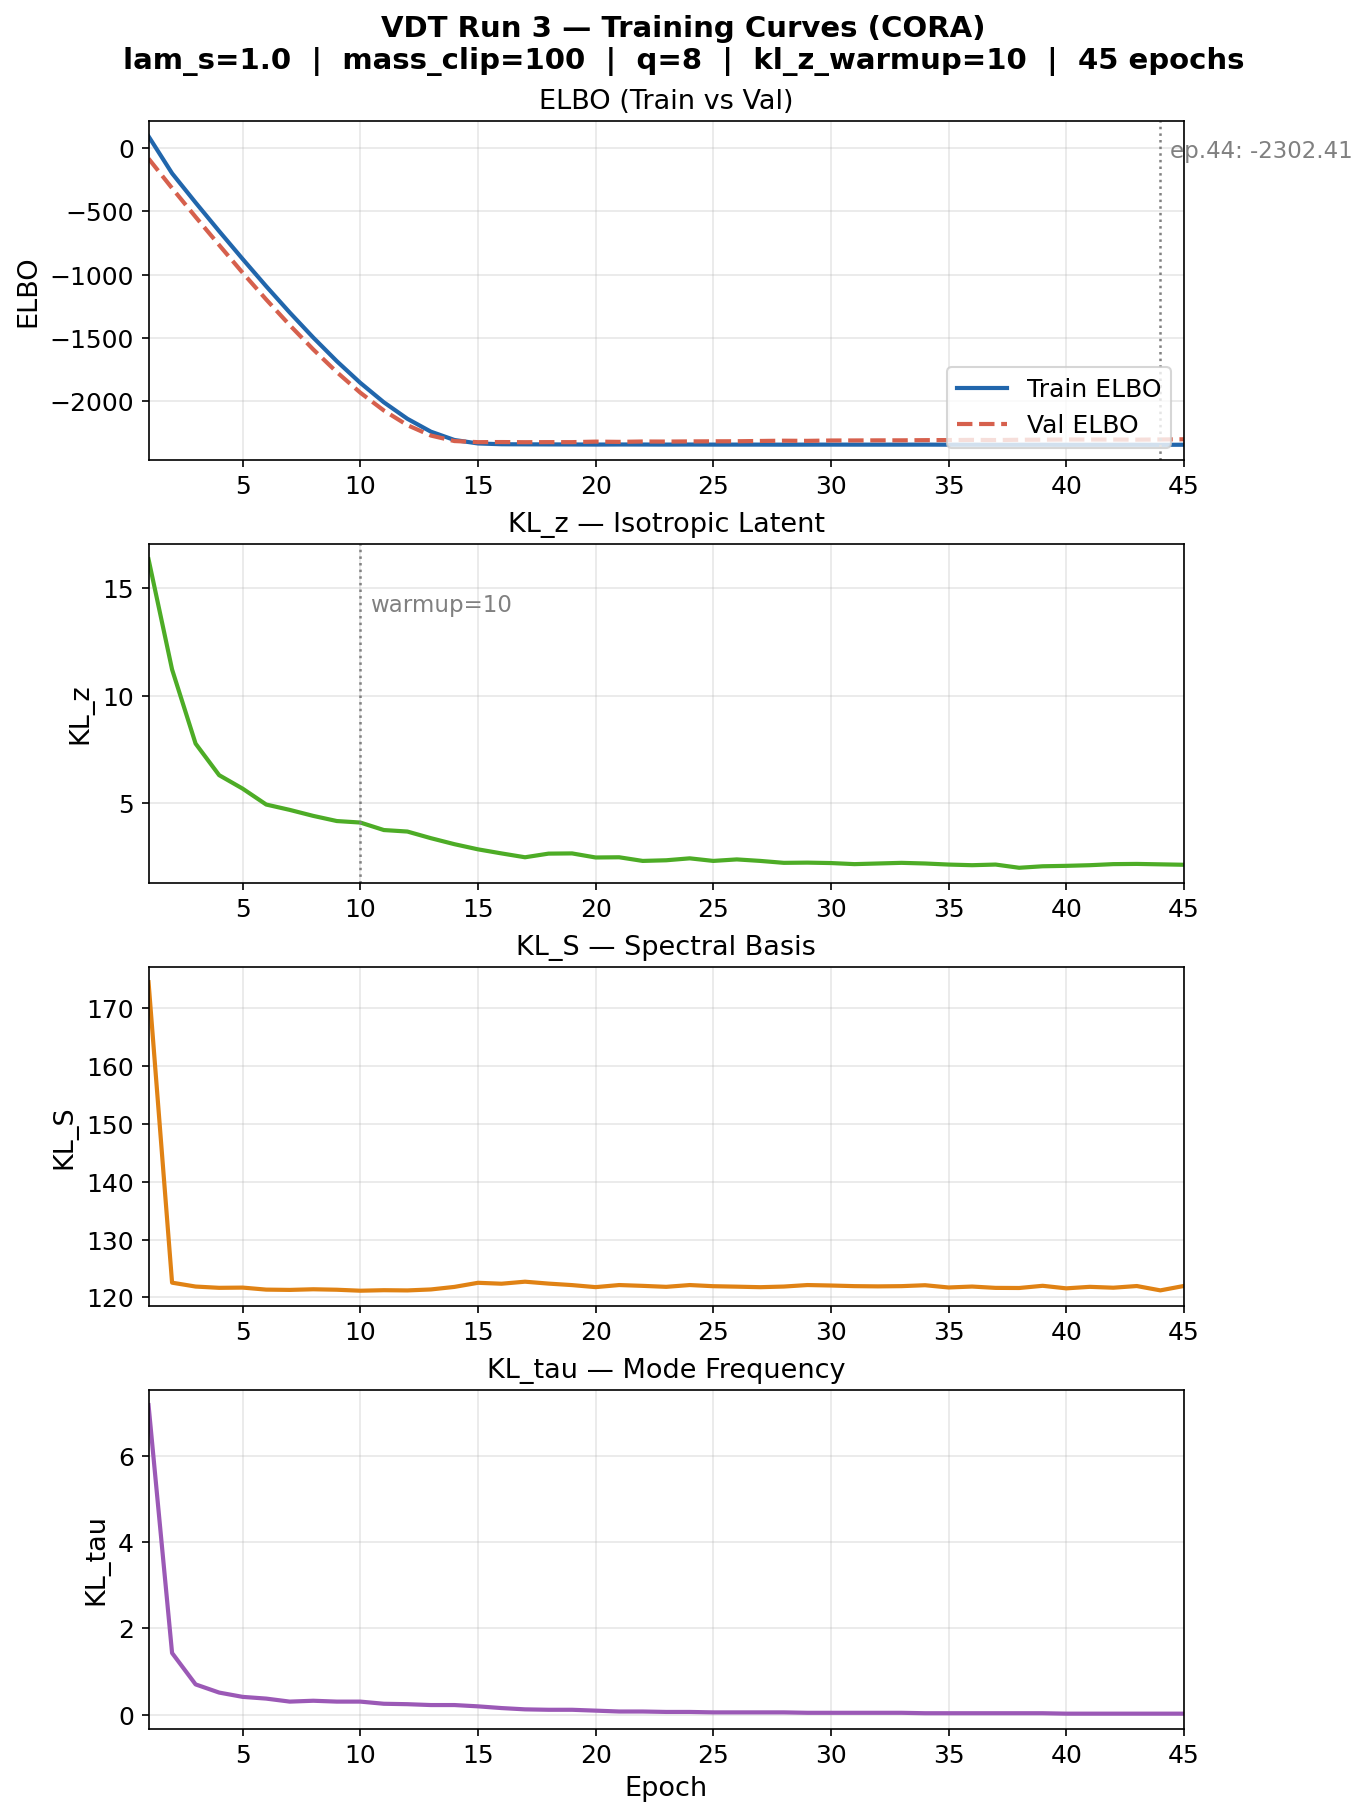
\includegraphics[width=0.65\textwidth]{../../docs/third-run-logs/training_curves.png}
  \caption*{\textbf{Run 3:} \texttt{lam\_s=1.0}, $q=8$, \texttt{kl\_z\_warmup=10}, 45 epochs}
\end{figure}

% ---- Run 4 ----
\begin{figure}[H]
  \centering
  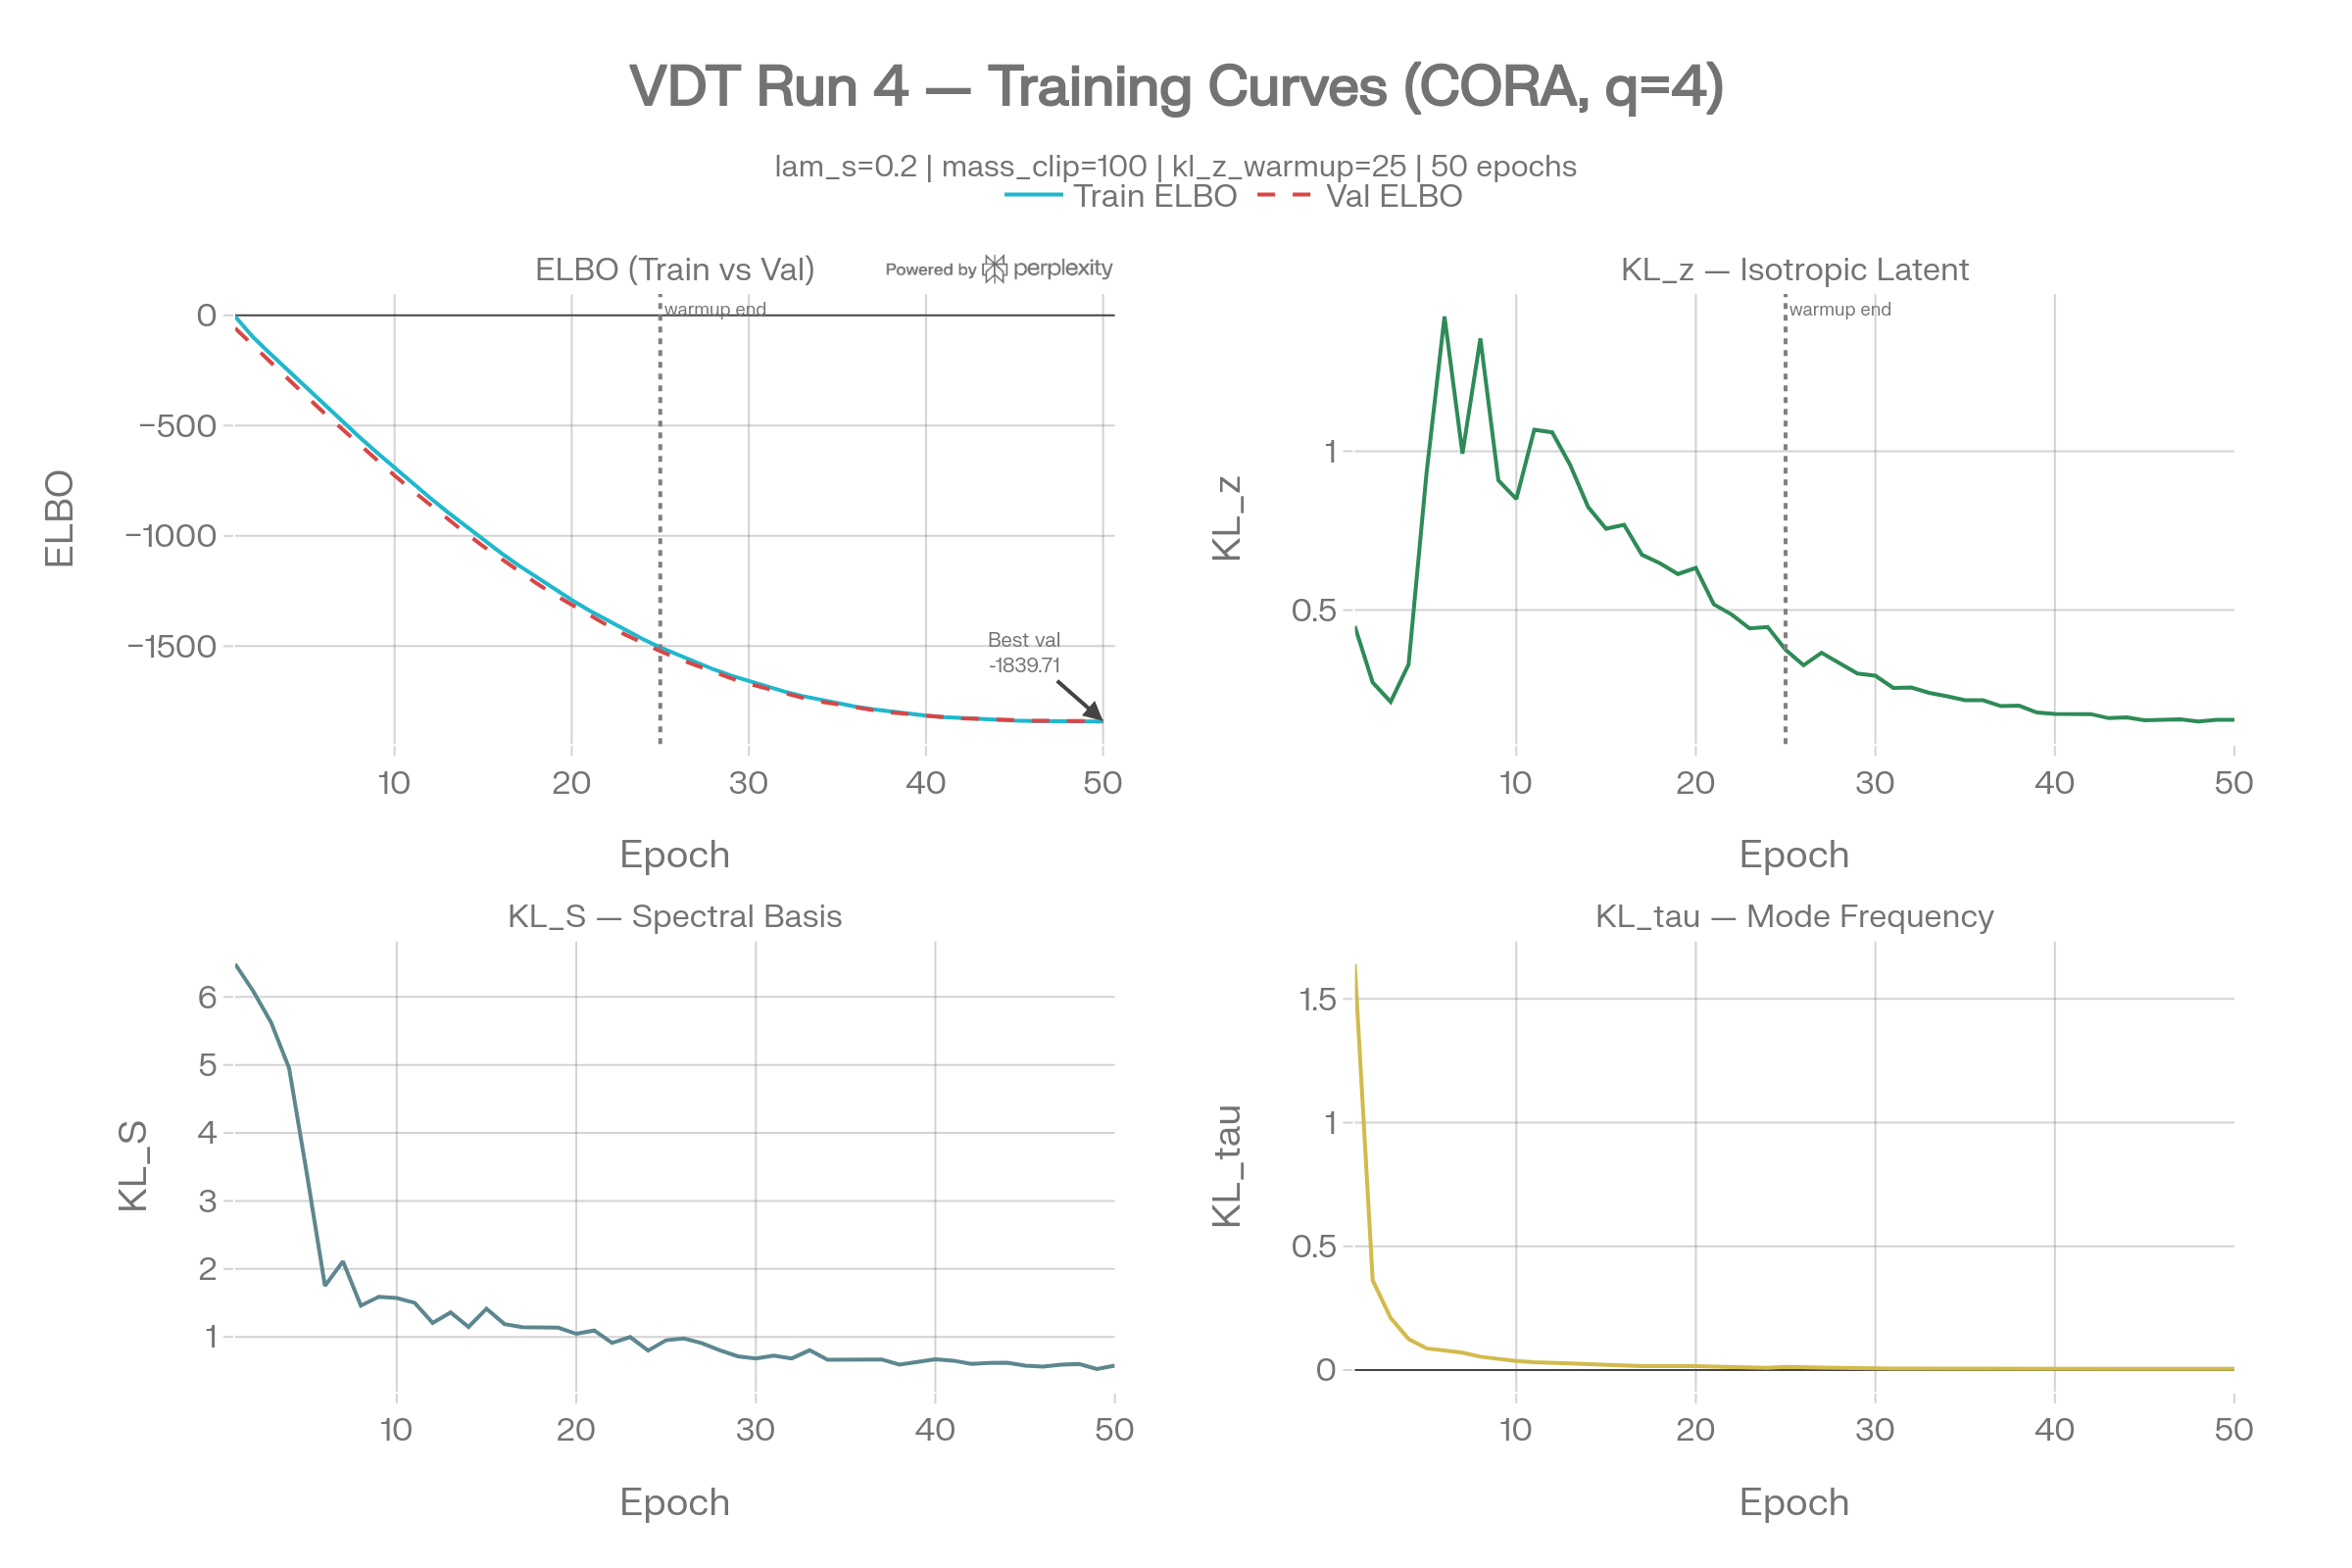
\includegraphics[width=0.65\textwidth]{../../docs/fourth-run-logs/training_curves.png}
  \caption*{\textbf{Run 4:} \texttt{lam\_s=0.2}, $q=4$, \texttt{kl\_z\_warmup=25}, 50 epochs}
\end{figure}

\begin{figure}[H]
  \centering
  \caption{Training and validation ELBO for Run~2 (top), Run~3 (centre),
    and Run~4 (bottom). Each panel shows ELBO, KL$_z$, KL$_S$, and KL$_\tau$
    over epochs. Run~3 shows KL$_S$ collapse to zero at epoch~10;
    Run~4 shows no plateau at epoch~50, suggesting continued improvement.}
  \label{fig:curves}
\end{figure}

Runs~2 and~3 show rapid ELBO improvement in epochs~1--15 followed by a
plateau (Figure~\ref{fig:curves}).
Run~4 does not plateau: the ELBO improves continuously across all 50 epochs,
with the train--val gap closing to fewer than 2 units by epoch~43, compared
to ${\approx}12$ units in Runs~2 and~3.
In all three runs the reconstruction loss accounts for more than 99\% of the
total ELBO at convergence, confirming that KL regularisation becomes
negligible relative to the reconstruction objective at this scale.

\subsection{Flagship Demo: Entropy-Controlled Spectral Generation}
\label{sec:experiments:demo}

Standard VAEs decode $\mathbf{z}$ into flat feature vectors; the VDT decodes
$\mathbf{z}$ into a \emph{graph wiring}---a Laplacian whose eigenvalues are
vibrational modes of the spring network (cf.\ Rayleigh~\cite{rayleigh1877}).
The latent space directly encodes spectral geometry, enabling samples whose
spectral entropy matches a target level.
This capability is unique to the VDT's vibrational latent representation and
is unavailable in flat-prior models.

Quantitative evaluation of entropy-controlled generation has not yet been
performed on any of the three completed runs: the synthetic spring network
benchmark, the natural test bed for spectral diversity, is deferred.
The persistent mode collapse across all runs indicates that the current latent
space does not yet perform discriminative spectral selection; meaningful
entropy-controlled sampling will require resolving the \texttt{active\_modes}
counter bug, tuning $\nu$ and $q_{\min}$, and evaluating on the spring dataset
where the entropy target is controllable by construction.
Run~4 is the most promising starting point: its continuous ELBO improvement
and tight train--val gap at epoch~50 suggest that a longer run at $q=4$,
\texttt{lam\_s=0.2} may achieve the spectral selectivity required.

% -----------------------------------------------------------------------
\section{Related Work}
\label{sec:related}
% -----------------------------------------------------------------------

\paragraph{Spectral graph autoencoders.}
Graph variational autoencoders~\cite{kipf2016} encode topology in the latent
space but do not use spectral priors.  VGAE and its successors decode
adjacency matrices directly, without a vibrational interpretation.

\paragraph{Probabilistic PCA on graphs.}
Laplacian Eigenmaps~\cite{belkin2003} and Diffusion Maps~\cite{coifman2006}
use the heat kernel for dimensionality reduction but are deterministic and
lack variational objectives.

\paragraph{NVIB.}
The Nonparametric Variational Information Bottleneck~\cite{nvib2022} applies
variational compression to sequence models.  The VDT shares the ELBO
philosophy but applies spectral-structural priors rather than capacity
constraints on a fixed-dimension latent.

\paragraph{Beta-VAE and disentanglement.}
Higgins et al.~\cite{higgins2017} introduce $\beta$-VAE, showing that
stronger KL regularisation encourages disentangled latent representations.
The VDT's eigenvalue-weighted spectral-basis KL can be seen as an
anisotropic generalisation of this pressure, tuning the regularisation
strength independently per spectral frequency band.

\paragraph{Real quantum mechanics.}
Renou et al.~\cite{renou2021} and McKague et al.~\cite{mckague2009} provide
experimental and theoretical grounding for real-valued quantum theories.
The VDT does not claim to \emph{be} a quantum system, but borrows the
structure of signed-amplitude interference as a computational primitive.

% -----------------------------------------------------------------------
\section{Discussion and Future Work}
\label{sec:conclusion}
% -----------------------------------------------------------------------

The VDT establishes a formal connection between three bodies of theory:
Rayleigh's vibrational mechanics, Aaronson's real-amplitude quantum
probabilities, and Bayesian graph-spectral learning.  The central
contribution is the four-term ELBO~\eqref{eq:elbo}, which replaces hard
spectral penalties with proper variational counterparts while preserving the
ArrowSpace wiring geometry.

A Spectral Diffusion improvement on this architecture is work in progress.

% -----------------------------------------------------------------------
\section*{Acknowledgements}
% -----------------------------------------------------------------------

The ArrowSpace computational library and the VDT codebase are developed and
maintained by the \href{https://github.com/sponsors/tuned-org-uk}{tuned-org-uk team}.
The architecture inherits the PPCA-to-VAE progression formalised in
\emph{The Little Book of Generative AI Foundations}~\cite{chen2026}.

The author acknowledges the use of AI-assisted tools during the preparation of this paper, including Perplexity for literature discovery, OpenAI GPT models for drafting and result analysis, NVIDIA Nemotron for exploratory formal verification analysis, and Claude Sonnet 4.6 for coding support and implementation checks~\cite{perplexity,openai_gpt5,nvidia_nemotron,anthropic_claude46}. All technical claims, interpretations, experiments, and final editorial decisions remain the sole responsibility of the authors.

\newpage

% -----------------------------------------------------------------------
% Bibliography
% -----------------------------------------------------------------------
\bibliographystyle{plain}
\begin{thebibliography}{99}

\bibitem{rayleigh1877}
Lord Rayleigh (J.W.S.\ Strutt).
\newblock \emph{The Theory of Sound}, Volumes I and II.
\newblock Macmillan, London, 1877/1894.

\bibitem{aaronson2013}
S.\ Aaronson.
\newblock \emph{Quantum Computing Since Democritus}, Chapter~9: Quantum.
\newblock Cambridge University Press, 2013.
\newblock \url{https://scottaaronson.com/democritus/lec9.html}

\bibitem{davis2026ldt}
L.~Davis, L.~Haller, A.~Alfarano, and M.~Santolucito.
\newblock Lattice Deduction Transformers.
\newblock \emph{arXiv:2605.08605}, 2026.
\newblock \url{https://arxiv.org/abs/2605.08605}

\bibitem{cousot1977}
P.~Cousot and R.~Cousot.
\newblock Abstract interpretation: a unified lattice model for static analysis of programs by construction or approximation of fixpoints.
\newblock In \emph{Proceedings of the 4th ACM Symposium on Principles of Programming Languages}, pages 238--252, 1977.

\bibitem{moriondo2026graphwiring}
L.~Moriondo, 
\newblock ``Graph Wiring: Eigenstructures for vector datasets and LLM operations,'' 
\newblock {\em TechArixiv}, 2026.
\newblock DOI: 10.36227/techrxiv.177220780.02840438.

\bibitem{moriondo2025arrowspace}
L.~Moriondo, 
\newblock ``ArrowSpace: introducing Spectral Indexing for vector search,'' 
\newblock {\em Journal of Open Source Software}, vol.~10, no.~113, p.~9002, 2025.
\newblock DOI: 10.21105/joss.09002.

\bibitem{moriondo2026vdeductive};
L.~Moriondo, 
\newblock ``Vibrational Deductive Transformer, Code and Analysis'' 
\href{https://github.com/tuned-org-uk/vibrational-deduction-transfomer}{%
    vibrational-deduction-transfomer}


\bibitem{chen2026}
T.~Chen,
\newblock ``The Little Book of Generative AI Foundations: An Intuitive Mathematical Primer,''
\newblock {\em arXiv preprint arXiv:2605.29713}, 2026.
\bibitem{chung1997}
F.R.K.\ Chung.
\newblock \emph{Spectral Graph Theory}.
\newblock AMS CBMS Monographs, 1997.
\newblock \url{https://mathweb.ucsd.edu/~fan/research/revised.html}

\bibitem{tipping1999}
M.E.\ Tipping and C.M.\ Bishop.
\newblock Probabilistic principal component analysis.
\newblock \emph{Journal of the Royal Statistical Society B}, 61(3):611--622, 1999.

\bibitem{kingma2013}
D.P.\ Kingma and M.\ Welling.
\newblock Auto-encoding variational Bayes.
\newblock \emph{arXiv:1312.6114}, 2013.
\newblock \url{https://arxiv.org/abs/1312.6114}

\bibitem{higgins2017}
I.\ Higgins et al.
\newblock $\beta$-VAE: Learning basic visual concepts with a constrained
  variational framework.
\newblock \emph{ICLR}, 2017.

\bibitem{belkin2003}
M.\ Belkin and P.\ Niyogi.
\newblock Laplacian Eigenmaps for dimensionality reduction and data
  representation.
\newblock \emph{Neural Computation}, 15(6):1373--1396, 2003.

\bibitem{coifman2006}
R.R.\ Coifman and S.\ Lafon.
\newblock Diffusion maps.
\newblock \emph{Applied and Computational Harmonic Analysis}, 21(1):5--30, 2006.

\bibitem{kipf2016}
T.N.\ Kipf and M.\ Welling.
\newblock Semi-supervised classification with graph convolutional networks.
\newblock \emph{arXiv:1609.02907}, 2016.

\bibitem{renou2021}
M.-O.\ Renou et al.
\newblock Quantum theory based on real numbers can be experimentally falsified.
\newblock \emph{Nature}, 600:625--629, 2021.

\bibitem{mckague2009}
M.\ McKague et al.
\newblock Simulating quantum systems using real Hilbert spaces.
\newblock \emph{Physical Review Letters}, 102:020505, 2009.

\bibitem{nvib2022}
K.\ Dib et al.
\newblock NVIB: Nonparametric variational information bottleneck.
\newblock \emph{arXiv}, 2022.

\bibitem{hopfield1982}
J.J.\ Hopfield.
\newblock Neural networks and physical systems with emergent collective
  computational abilities.
\newblock \emph{PNAS}, 79(8):2554--2558, 1982.

\bibitem{einstein1905}
A.\ Einstein.
\newblock {\"U}ber die von der molekularkinetischen Theorie der W{\"a}rme
  geforderte Bewegung von in ruhenden Fl{\"u}ssigkeiten suspendierten Teilchen.
\newblock \emph{Annalen der Physik}, 322(8):549--560, 1905.

\bibitem{jaynes1957}
E.T.\ Jaynes.
\newblock Information theory and statistical mechanics.
\newblock \emph{Physical Review}, 106(4):620--630, 1957.

\bibitem{hu2020}
W.\ Hu et al.
\newblock Open Graph Benchmark: Datasets for machine learning on graphs.
\newblock \emph{NeurIPS}, 2020.

\bibitem{perplexity}
Perplexity AI (2026).
\newblock Perplexity.
\newblock \url{https://www.perplexity.ai}.

\bibitem{openai_gpt5}
OpenAI (2025).
\newblock GPT-5.

\bibitem{anthropic_claude46}
Anthropic (2026).
\newblock Claude sonnet 4.6.
\newblock \url{https://www.anthropic.com/claude/sonnet}.

\bibitem{nvidia_nemotron}
NVIDIA (2026).
\newblock NVIDIA nemotron AI models.
\newblock \url{https://developer.nvidia.com/nemotron}.

\end{thebibliography}

\end{document}
